\subsection{Shift-Left Modelle}
\label{sec:arten}
Der Shift-Left-Gedanke ist eine grundsätzliche Herangehensweise, die sich auf die meisten Konzepte und Modelle anwenden lässt. Da dieser Beitrag sich auf die Verbindung von agilen Methoden und Security durch den Shift-Left-Ansatz konzentriert, werden im Folgenden zwei Shift-Left-Modelle erklärt, die dabei behilflich sind.

\begin{figure}
    \centering
    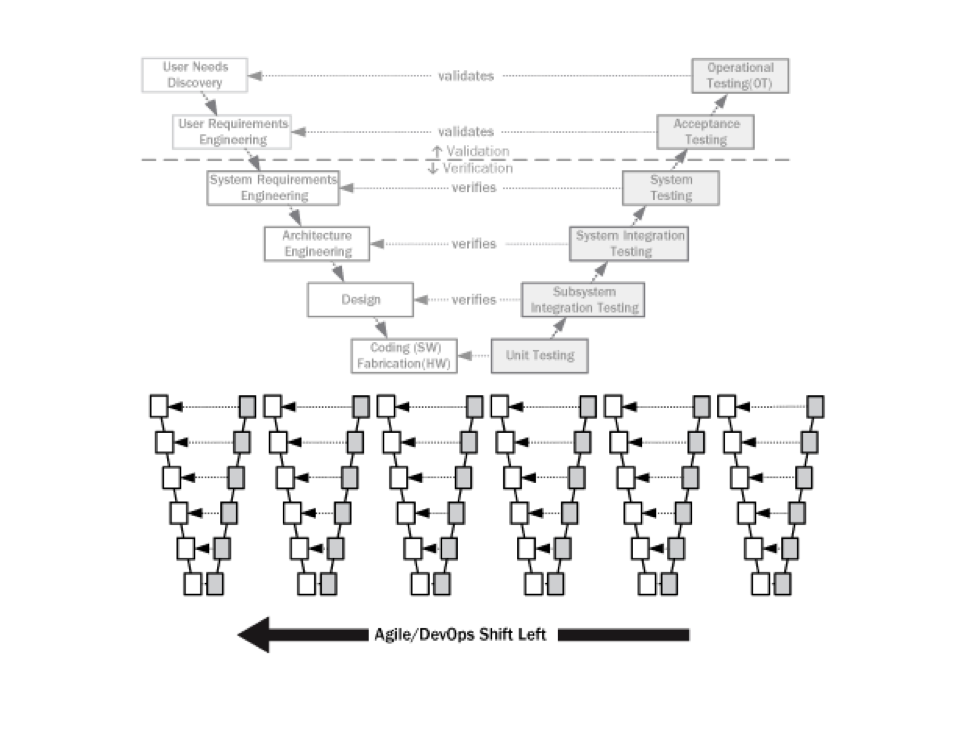
\includegraphics[width=0.9\linewidth]{images/Agile_DevOps_Shift_Left.png}
    \caption{Agile/DevOps Shift Left \cite{firesmith_four_2015}}
    \label{fig:agiledevops}
\end{figure}

Das erste Modell ist das \textit{Agile/DevOps Shift-Left-Testing}. Zur Erklärung des Modells dient die Abbildung \ref{fig:agiledevops}. Ausgangslage für die Grafik ist das traditionelle V-Modell, welches verblasst in der oberen Hälfte von Abbildung \ref{fig:agiledevops} zu erkennen ist. Die mehrfachen Vs darunter visualisieren die Arbeitsweise im agilen Bereich. Jedes V stellt einen Zyklus der Entwicklung dar, der beim agilen Arbeiten meist \textit{Sprint} genannt wird \cite{rani_shift-left_2023}. Diese Aufteilung nutzt bereits eine Implementierung des Shift-Left-Ansatzes. Durch das Aufteilen eines gesamten Projekts in mehrere kleine Zyklen werden beispielsweise Tests in jedem Zyklus umgesetzt \cite{rani_shift-left_2023}. Betrachtet man die gesamte Laufzeit eines Projekts, werden Tests dadurch automatisch nicht erst am Ende des gesamten Projekts implementiert \cite{bjerke-gulstuen_high_2015}. Agile/DevOps Shift-Left-Testing schlägt weiterhin vor, den Fokus auf das Testing in frühere Sprints zu verstärken \cite{bjerke-gulstuen_high_2015}. Dabei ist das Automatisieren dieser Tests ein ausschlaggebendes Prinzip im DevOps-Bereich \cite{rani_shift-left_2023}. Shift-Left will diese Automatisierung nutzen, um das kontinuierliche Testen bereits als Bestandteil in die frühen Entwicklungsphasen zu integrieren \cite{rani_shift-left_2023}. Die frühzeitige Nutzung von CI/CD und DevOps hilft dabei, Fehler und Sicherheitslücken rechtzeitig zu erkennen und somit langfristige Kosten zu sparen \cite{rani_shift-left_2023}. Eine effektive Methode, um Tests für Sicherheitslücken bzw. -probleme zu automatisieren, ist die Nutzung von SAST und DAST, welche später genauer analysiert werden. Eine weitere Eigenschaft, die durch die agile Herangehensweise und Shift-Left gestärkt wird, ist die Zusammenarbeit und Kommunikation zwischen Development- und Testing-Teams \cite{rani_shift-left_2023}. Durch die Parallelisierung beider Prozesse gibt es einen höheren Austausch an Feedback, wodurch auf Fehler schnell reagiert werden kann. Vor allem bei Projekten mit hohen Sicherheitsanforderungen wird dadurch das Bewusstsein für Sicherheit bei allen Beteiligten gestärkt \cite{dawoud_better_2024}.

Der zweite Ansatz, der hier vorgestellt werden soll, ist das \textit{Model-Based Shift-Left Testing (MBSLT)}. Wie zuvor veranschaulicht Abbildung \ref{fig:modelbased} die Herangehensweise für das MBSLT basierend auf dem V-Modell. Anders als der Agile/DevOps-Ansatz fokussiert sich MBSLT auf das Testen des gesamten Modells und nicht auf den Quellcode des Projektes \cite{rani_shift-left_2023}. In \ref{fig:modelbased} ist zu erkennen, dass neben jedem standardmäßigen Schritt des V-Modells ein paralleler Schritt erfolgt, der darauf abzielt, das Systemmodell zu testen. Diese Systemmodelle werden beispielsweise durch UML oder Datenflussdiagramme dargestellt \cite{rani_shift-left_2023}. Basierend darauf werden Tests erstellt, um Schwachstellen in der Architektur- und Design-Ebene zu erkennen. Auch diese Art von Tests kann durch CI/CD automatisiert werden \cite{rani_shift-left_2023}. MBSLT hilft dabei, potenzielle Fehler noch vor der Implementierung zu erkennen, wodurch spätere Kosten vermieden werden können \cite{rani_shift-left_2023}. Des Weiteren wird die Anforderungsanalyse verbessert, da MBSLT sicherstellt, dass Anforderungen vollständig und konsistent sind \cite{rani_shift-left_2023}. Dieser Vorteil trägt somit auch zur besseren Kommunikation zwischen dem Development-, Testing- und Security-Team bei.

\begin{figure}
    \centering
    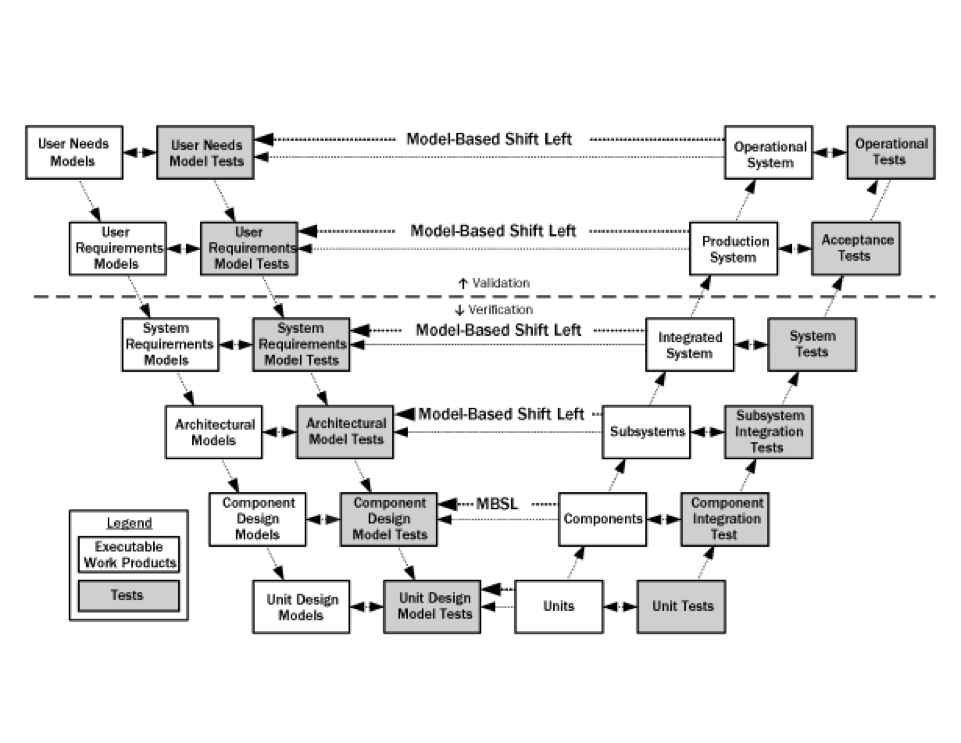
\includegraphics[width=0.9\linewidth]{images/Model_Based_Shift_Left.png}
    \caption{Model-Based Shift Left \cite{firesmith_four_2015}}
    \label{fig:modelbased}
\end{figure}

